\section{Nurul Izza Hamka (1174062)}
\subsection{Instalasi Map Server}
\begin{enumerate}
    \item Langkah pertama pertama  adalah menginstall MapServer (MS4W)
  \hfill\break
  \begin{figure}[H]
  
\includegraphics[width=4cm]{figures/tugas4/1174062/1.png}
  \centering
  \caption{Gambar Link Download MS4W}
  \end{figure}
    
    \item Setelah itu klik file seperti pada gambar dibawah ini untuk di download
    
  \hfill\break
  \begin{figure}[H]
  
\includegraphics[width=4cm]{figures/tugas4/1174062/2.png}
  \centering
  \caption{Gambar Untuk Install File exe}
  \end{figure}
  
    \item Setelah itu run MS4W yang telah didownload untuk melanjutkan instalasi
    
  \hfill\break
  \begin{figure}[H]
  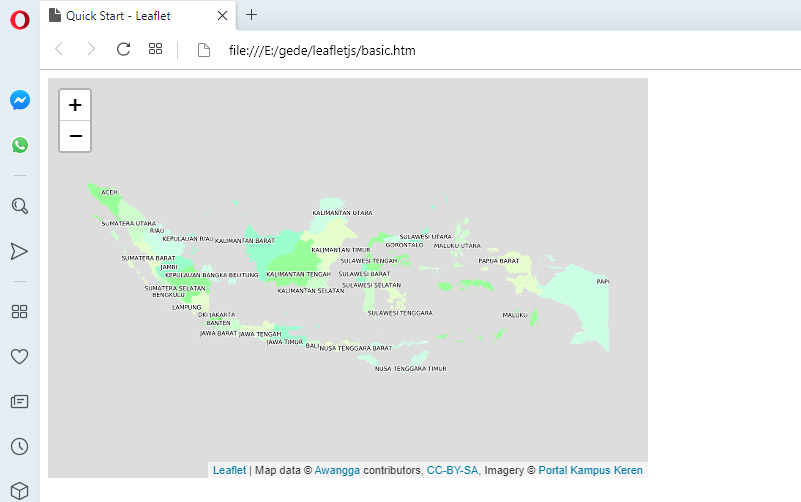
\includegraphics[width=4cm]{figures/tugas4/1174062/3.png}
  \centering
  \caption{Gambar Proses Instalasi Ms4w}
  \end{figure}
  
\end{enumerate}

\subsection{Konfigurasi Map Server}
Langkah selanjutnya setelah proses intalasi, maka kita akan melakukan konfigurasi
\begin{enumerate}
  \item Buka folder ms4w. Masuk ke folder apache, kemudian masuk ke folder conf dan pilih file httpd.conf
\hfill\break
  \begin{figure}[H]
  
\includegraphics[width=4cm]{figures/tugas4/1174062/5.png}
  \centering
  \caption{Gambar Untuk File http.conf}
  \end{figure}
  
  \item Buka file httpd.conf dan ubah listen port nya menjadi port 80.
  
\hfill\break
  \begin{figure}[H]
  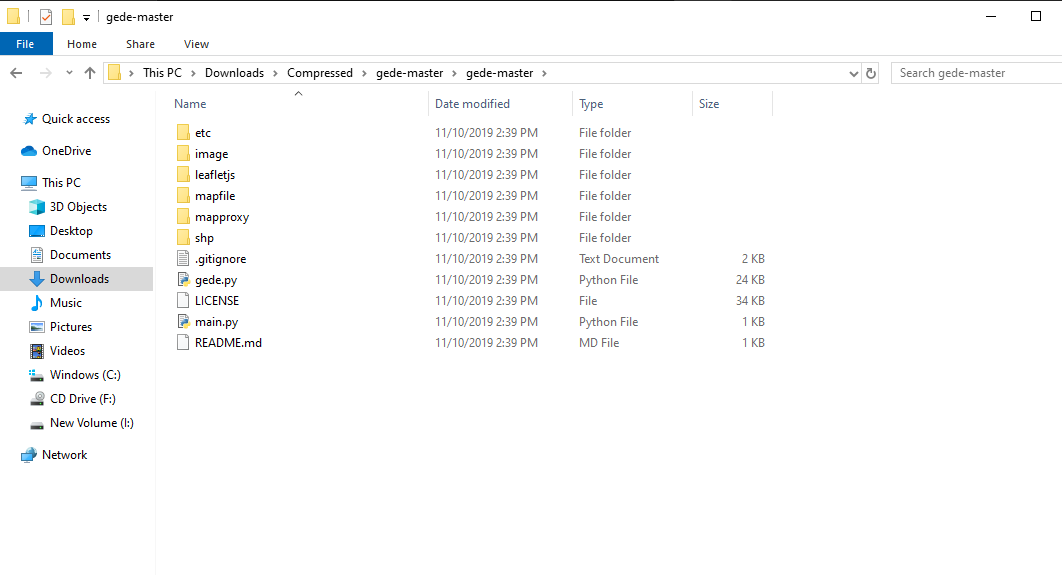
\includegraphics[width=4cm]{figures/tugas4/1174062/6.png}
  \centering
  \caption{Gambar Listen port 80}
  \end{figure}
  
  \item Kemudian klik windows + r dan ketikan perintah services.msc
    
\hfill\break
  \begin{figure}[H]
  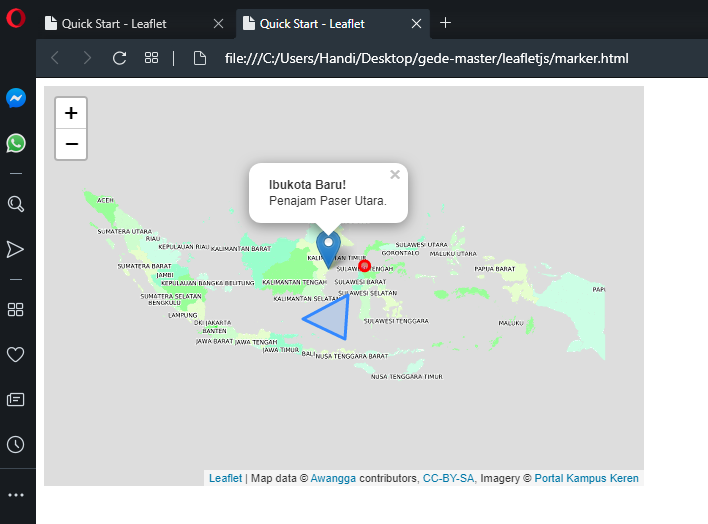
\includegraphics[width=4cm]{figures/tugas4/1174062/7.png}
  \centering
  \caption{Gambar Untuk Mengakses Halaman Service}
  \end{figure}
  
  \item Kemudian Pilih MS4W untuk Web Server, kemudian Klik OK
 \hfill\break
  \begin{figure}[H]
  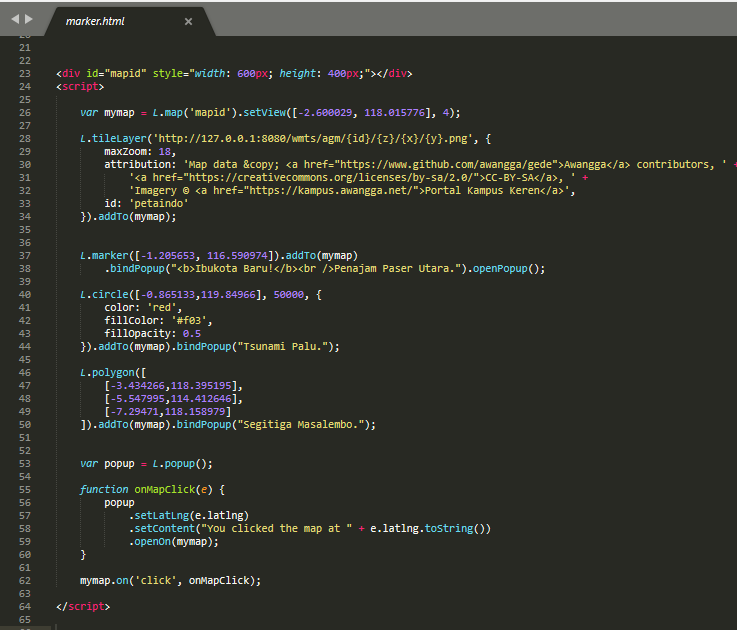
\includegraphics[width=4cm]{figures/tugas4/1174062/4.png}
  \centering
  \caption{Gambar Untuk Mengakses Halaman Service}
  \end{figure}
  
\subsection{Pengujian}
\begin{enumerate}
	\item Setelah dilakukan Konfigurasi maka kita akan melakukan pengujian, ada dua file yang dibutuhkan yaitu .map dan .ymal
  \item Pertama masuk ke web dengan Link https://github.com/awangga/gede/

 \hfill\break
  \begin{figure}[H]
  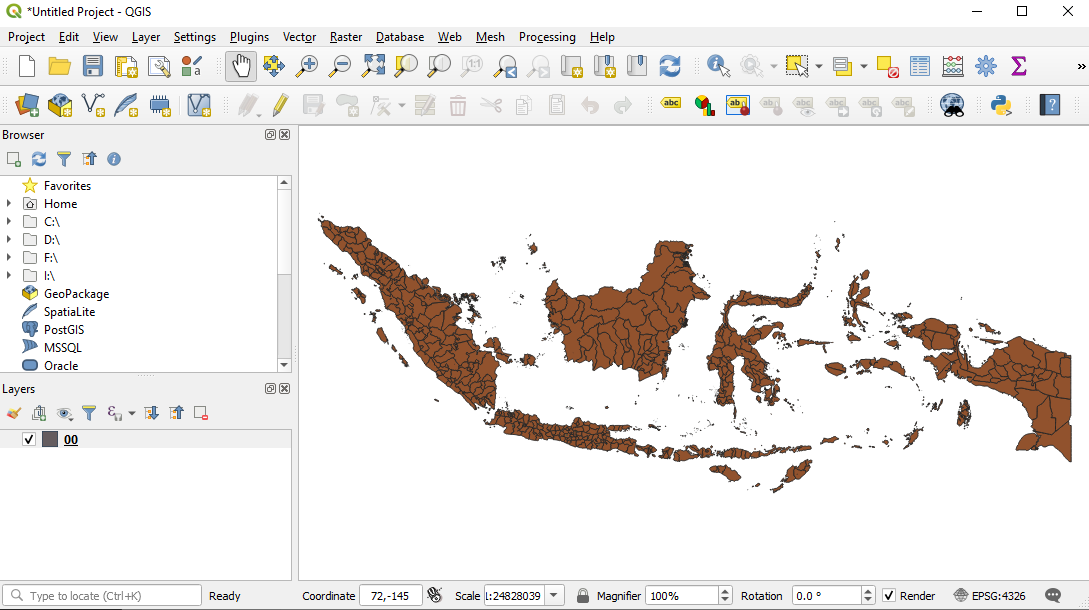
\includegraphics[width=4cm]{figures/tugas4/1174062/8.png}
  \centering
  \caption{Link Github}
  \end{figure}


  \item Kemudian file Clone atau Download, selanjutnya Download ZIP
  
    \hfill\break
    \begin{figure}[H]
  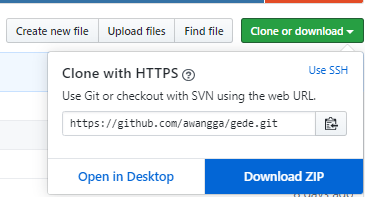
\includegraphics[width=4cm]{figures/tugas4/1174062/9.png}
  \centering
  \caption{Gambar Untuk Download File}
  \end{figure}

  \item Kemudian buka file agm.ymal  pada file yang telah didownload tadi untuk meyesuaikan file directori kita
    
    \hfill\break
    \begin{figure}[H]
  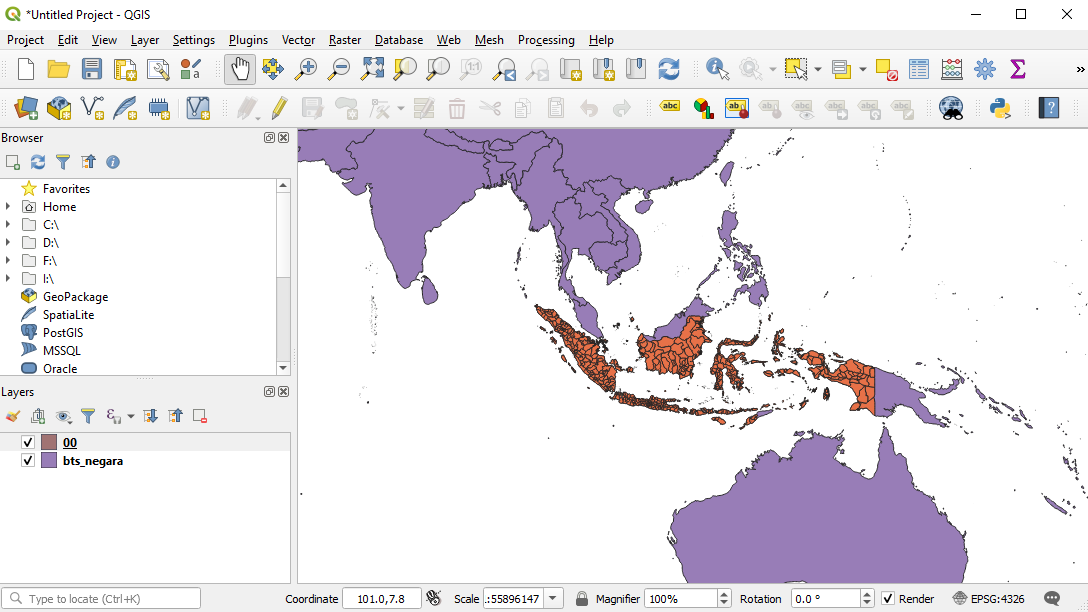
\includegraphics[width=4cm]{figures/tugas4/1174062/10.png}
  \centering
  \caption{Gambar di File aqm.ymal}
  \end{figure}
  
   \item Selajutnya buka app QGIS
  
 \hfill\break
    \begin{figure}[H]
  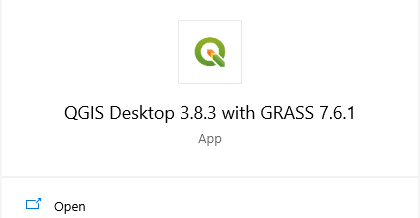
\includegraphics[width=4cm]{figures/tugas4/1174062/11.png}
  \centering
  \caption{Gambar Untuk Aplikasi QGIS}
  \end{figure}
  
  \item Selajutnya buka File 00.shp 
  
 \hfill\break
    \begin{figure}[H]
  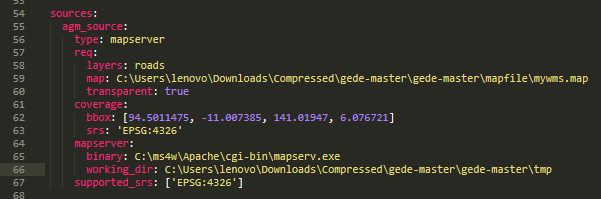
\includegraphics[width=4cm]{figures/tugas4/1174062/12.png}
  \centering
  \caption{Gambar Hasil 00.shp}
  \end{figure}

 \item Selajutnya jalankan file bts negara.shp
   
 \hfill\break
    \begin{figure}[H]
  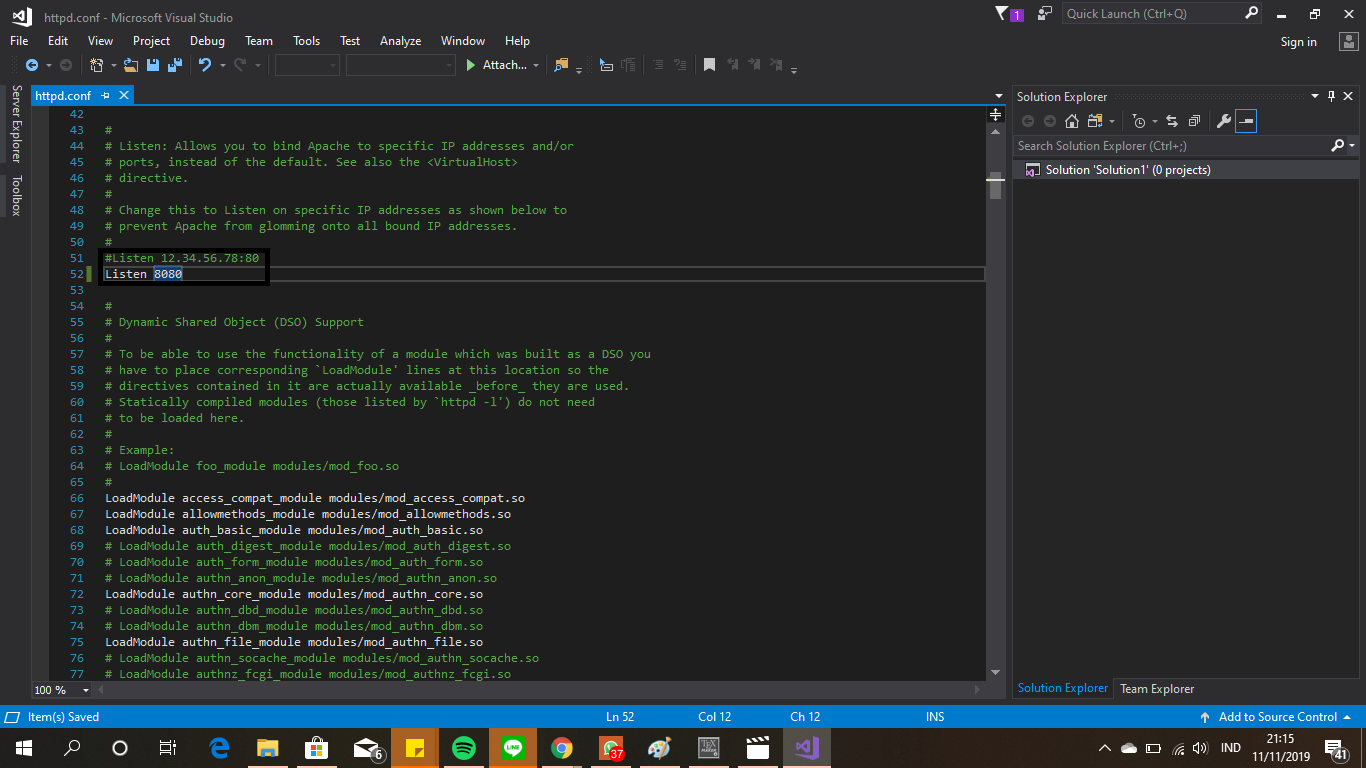
\includegraphics[width=4cm]{figures/tugas4/1174062/13.png}
  \centering
  \caption{Gambar Hasil bts negara.shp}
  \end{figure}
 
\end{enumerate}
\subsection{Link Youtube Instalasi MapServer}
{https://www.youtube.com/watch?v=BkFsJXB1vJ8}

\subsection{Instalasi MapProxy}
\begin{enumerate}
  \item Pertama buka Command Prompt
  \item Lalu ketikkan pip install MapProxy
  \hfill\break
  \begin{figure}[H]
  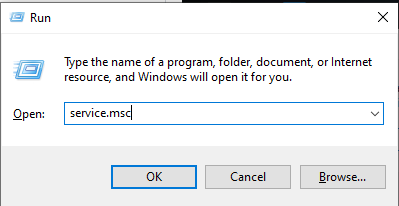
\includegraphics[width=4cm]{figures/tugas4/1174062/14.png}
  \centering
  \caption{Instalasi MapProxy}
  \end{figure}

\end{enumerate}

\subsection{Link Youtube MapProxy dan Menjalankannya}
https://www.youtube.com/watch?v=E8SSxJZm9k8